\documentclass{article}
\usepackage{amsmath}
\usepackage{tikz}
\usetikzlibrary{positioning}

\begin{document}

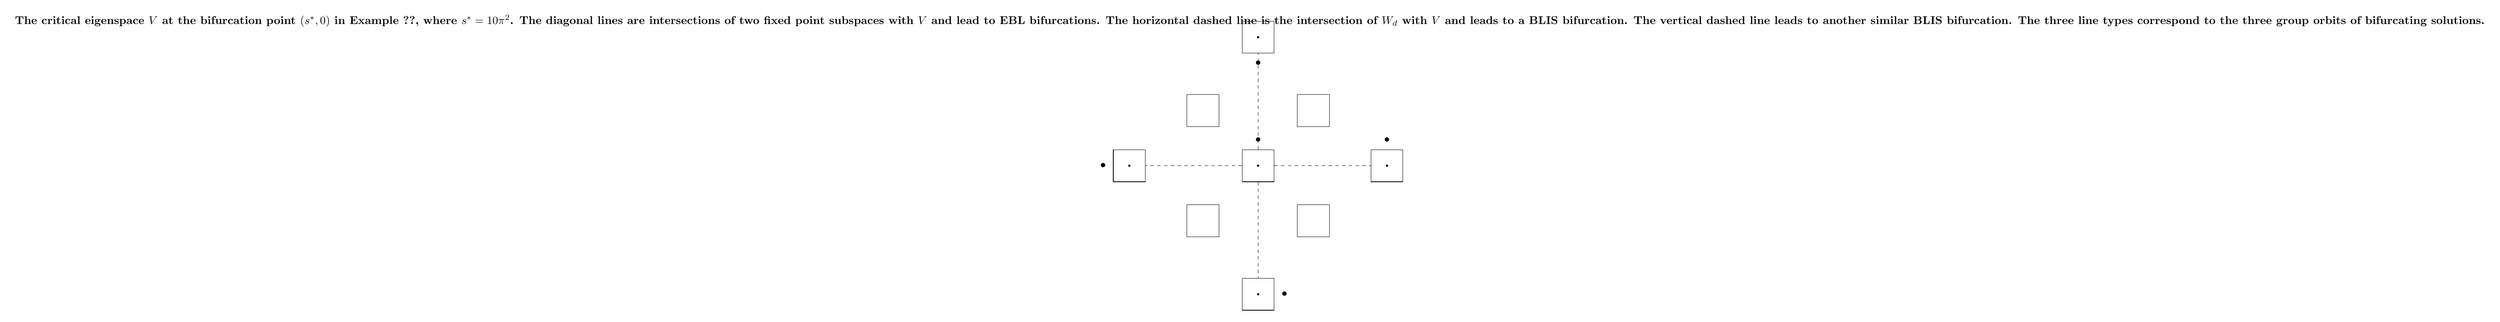
\begin{tikzpicture}[node distance=1cm]
    % Define styles for the nodes
    \tikzstyle{block} = [draw, fill=white, rectangle, 
        minimum height=10mm, minimum width=10mm, text centered]

    \node[block] (A) {};
    \node[block, above right=of A] (B) {};
    \node[block, below right=of A] (C) {};
    \node[block, below left=of A] (D) {};
    \node[block, above left=of A] (E) {};
    \node[block, right=3cm of A] (F) {};
    \node[block, left=3cm of A] (G) {};
    \node[block, below=3cm of A] (H) {};
    \node[block, above=3cm of A] (I) {};

    % Draw the connecting lines
    \draw[dashed] (A) -- (F);
    \draw[dashed] (A) -- (G);
    \draw[dashed] (A) -- (H);
    \draw[dashed] (A) -- (I);

    % Add dots at the intersections
    \fill (A) circle (1pt);
    \fill (F) circle (1pt);
    \fill (G) circle (1pt);
    \fill (H) circle (1pt);
    \fill (I) circle (1pt);

    % Labels for the dots
    \node[above=1mm of A] {$\bullet$};
    \node[above=1mm of F] {$\bullet$};
    \node[left=1mm of G] {$\bullet$};
    \node[right=1mm of H] {$\bullet$};
    \node[below=1mm of I] {$\bullet$};

    % Add annotations
    \node at (current bounding box.north) {\textbf{The critical eigenspace $V$ at the bifurcation point $(s^*,0)$ in Example~\ref{exa:lambda13}, where $s^*=10\pi^2$. The diagonal lines are intersections of two fixed point subspaces with $V$ and lead to EBL bifurcations. The horizontal dashed line is the intersection of $W_d$ with $V$ and leads to a BLIS bifurcation. The vertical dashed line leads to another similar BLIS bifurcation. The three line types correspond to the three group orbits of bifurcating solutions.}};
\end{tikzpicture}

\end{document}